\documentclass[a4paper,12pt]{article}
% Package to make citations superscript with brackets
\usepackage[numbers]{natbib}
% Package to change margin size
\usepackage{anysize}
\marginsize{2cm}{2cm}{1cm}{2cm}
% Package to make headers
\usepackage{fancyhdr}
\renewcommand{\headrulewidth}{0pt}
% Package for highlights
\usepackage{soul}
% Colours for the references links
\usepackage[dvipsnames]{xcolor}
% Package to link references
\usepackage{hyperref}
\usepackage{graphicx}
\usepackage{float}
\usepackage[italian]{babel}
\hypersetup{
    colorlinks=true,
    linkcolor=black,
    citecolor=CadetBlue,
    filecolor=CadetBlue,      
    urlcolor=CadetBlue,
}
% Package for lorem ipsum
\usepackage{lipsum}
% Package for multicolumn
\usepackage{multicol}

% Packages for formulas, chemistry and units
\usepackage{physics, mhchem, siunitx}

\usepackage{cleveref} % clever references
\crefname{table}{tab.}{tab.}

\usepackage{multicol,caption,subcaption}
% Package for removing paragraph indentations
\usepackage{parskip}
\usepackage{siunitx}
\sisetup{separate-uncertainty = true} % errori: posso scrivere \SI{20(8)}{\meters}
\setlength\columnsep{18pt} 
\setlocalecaption{italian}{figure}{Fig.}
\setlocalecaption{italian}{table}{Tab.}
\counterwithin{figure}{section} % comandi per numerazione interna di figure, tabelle ed equazioni
\counterwithin{table}{section}
\counterwithin{equation}{section}

% latex command utils
\newcommand{\newsec}[1]{
\vspace{0.3cm}
{\color{gray}\hrule}
\begin{center}
\section{#1}
\bigskip
\end{center}
{\color{gray}\hrule}
\vspace{0.1cm}
}

\newcommand{\help}[1]{\textcolor{red}{\bfseries [#1]}}
 
\begin{document}
\begin{center}

\small{Corso di Struttura della Materia con Laboratorio, A.A. 2025-26} \\
\vspace{0.4cm}
\small{\textbf{Relazione Tecnica di Laboratorio}}\\
\vspace{0.4cm}
\LARGE{\textbf{Esperienza: Raggi X}}
\vspace{0.4cm} \\
\normalsize{Massimiliano Moro, Rémi Roux, Luca Tempesta, Simone Vallauri} \\
\vspace{0.1cm}
\small (gruppo C1) \\

\vspace{0.1cm}
\medskip
\normalsize
\end{center}
\vspace{0.4cm}
{\color{gray}\hrule}
\medskip

\begin{abstract}
\noindent Studiamo lo spettro di emissione $ \gamma $ di varie sorgenti radioattive come \ce{^60Co}, \ce{^137Cs}, \ce{^22Na} etc. misurando la radiazione ocn uno scintillatore del tipo \ce{NaI(Tl)}. Osservando la posizione dei picchi decretiamo il processo che origina l`emissione osservata, caratterizziamo la presenza di elementi radioattivi in una roccia di origine ignota e lo spettro emissivo del fondo ambientale. Studiamo la risoluzione del rivelatore al variare dell`energia osservata stimandola a $ R = 6.5\% $, e successivamente misuriamo l`attività di una sorgente di tipo \ce{^137Ce} con metodo relativo e assoluto. Infine determiniamo il coefficiente di assorbimento di massa $ \mu / \rho = (0.1040 ± 0.0010)$ \unit{cm^2/g} compatibile al $ 5\% $ con il valore teorico considerato.

\end{abstract}

\tableofcontents
\clearpage

\pagestyle{fancy}
\fancyhead{} % clear all header fields
\fancyhead[L]{\small Struttura della Materia}
\fancyhead[C]{\small \bfseries Raggi X}
\fancyhead[R]{\small gruppo C1}

\section{Introduzione all'esperienza}
Vogliamo studiare le caratteristiche del decadimento gamma di diversi isotopi radioattivi e dell'interazione tra raggi gamma e materia. 
L'interesse nello studio deriva dai risultati ottenuti che forniscono informazioni utili sulla struttura nucleare atomica e sui numeri quantici ad essa relativi.
Per effettuare uno studio precisoi useremo dei rivelatori \ce{NaI(Tl)} letti da un fotomoltiplicatore.

\subsection{sezioni}
\begin{itemize}
    \item proprietà della catena elettronica di misura?
    \item calibrazione multicanale
    \item studio di sorgenti \ce{^137Cs} \ce{^60Co} \ce{^22Na} \ce{^57Co}
    \item identificazione elementi radioattivi in rocce e fondo ambientale (analisi gamma)
    \item risoluzione del rivelatore, misura FWHM di \ce{^137Cs} \ce{^60Co} \ce{^22Na}
    \item misura relativa e assoluta dell'attività di una sorgente
    \item misura assorbimento gamma nel \ce{Pb}, determinazione coeff. $\mu$ assorb. massa
    \item effetti di somma nello spettro di \ce{^60Co} (struttura livelli nucleo figlio)

\end{itemize}

\section{postazione A e apparecchiatura}

La postazione usa come rivelatore un cristallo di \ce{NaI(Tl)} di diametro $ 2^{"} = 50.8 mm $ letti da fotomoltiplicatori. Nello specifico la nostra posizione usa moduli NIM per alimentare i fotomoltiplicatori e l'elettronica di amplificazione, questa configurazione ci permette di studiare il segnale del fotomoltiplicatore con un oscilloscopio.
\begin{center}
    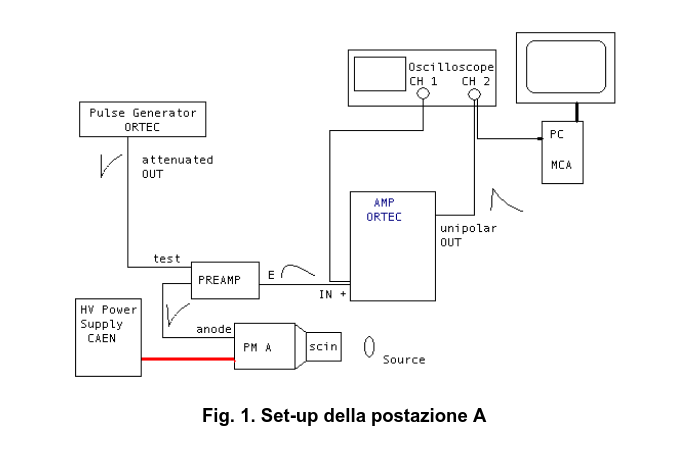
\includegraphics[scale=0.5]{images/setup_A}
\end{center}

Attenzione:
\begin{itemize}
    \item Manipolare le sorgenti con le apposite pinzette e lasciare le sorgenti nella cassetta di piombo per tutta l'esperienza
    \item ogni rivelatore ha una tensione massima (HV) da rispettare per mantenere l'integrità dei componenti (impostare a 0 prima di uscire dal programma di acquisizione)
    \item lasciare invariata la posizione delle mattonelle di piombo (tossico per ingestione)
\end{itemize}


\subsection{Setup e verifica impostazioni}
Abbiamo verificato il corretto funzionamento della postazione e verificato che la posizione sul canale $ \sim 780 $ fosse relativa al picco ad energia maggiore per la sorgente \ce{^60Co}, variando la tensione fornita al fotomoltiplicatore e/o il guadagno dell'amplificatore. Questa procedura serve per garantire il rientro nel range del multicanale per le misure successive.

\section{Studio della catena elettronica di misura}

In questa sezione, prima di raccogliere dati sullo spettro energetico relativo a differenti sorgenti radioattive, vogliamo verificare la linearità della catena elettronica di misura.
A tal proposito abbiamo raccolto dati sufficienti a costruire due grafici che illustrassero le proprietà cercate.
Gli strumenti utilizzati per misurare le quantità riportate sono un generatore di impulsi, un oscilloscopio ed un analizzatore multicanale.
Il valori del canale del picco acquisito, la $ V_{in} $ in entrata e la $ V_{out} $ in uscita all'amplificatore sono riportati nei grafici seguenti.
Come evidente dai parametri calcolati la risposta è lineare come ci aspettavamo.

\begin{center}
    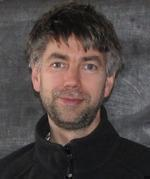
\includegraphics{images/pacini}
    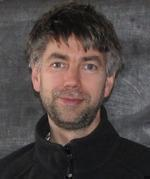
\includegraphics{images/pacini}
\end{center}

\section{Acquisizione degli spettri}

Abbiamo acquisito una serie di $ 8 $ misurazioni della durata di $ 2 $ \unit{min} ciascuna per \ce{^60Co} e \ce{^137Cs}.
Per caratterizzare entrambe le sorgenti abbiamo raccolto la posizione del centroide del picco fotoelettrico e la sua FWHM, come riportato dal software di acquisizione, selezionando un intervallo di canali che a priori contenesse il picco interessato (ROI).\\
Dopo l'acquisizione spettroscopica per tutti i tipi di sorgente a disposizione, abbiamo acquisito nuovamente lo spettro della sorgente iniziale per verificare che il guadagno del sistema fosse rimasto costante.
Posizionando infine il rivelatore al di fuori della schermatura di piombo, senza sorgenti, abbiamo misurato per $ \sim 1 $ \unit{ora} lo spettro del fondo ambientale.

\subsection{Calibrazione del multicanale}

Usando picchi di sorgenti note abbiamo calibrato il multicanale, identificato la posizione del centroide relativo al picco fotoelettrico di ogni sorgente e graficato i risultati in energia-canali. Abbiamo convertito il valore (CHN) in E(CHN) grazie alla funzione relativa \help{(riportare)}, per il calcolo degli errori \help{(riportare)}. 

\section{Spettroscopia di varie sorgenti gamma}
Analizzando le misure raccolte per gli spettri delle varie sorgenti (eccetto \ce{^57Co}), abbiamo identificato le caratteristiche principali che ci permettono di risalire a che tipo di emissione gamma stiamo osservando.

\begin{itemize}
    \item picchi fotoelettrici: assorbimento totale del fotone da parte del cristallo
    \item spalle compton: assorbimento di energia per effetto Compton da parte dell'elettrone prodotto nel cristallo
    \item backscattering: raggi gamma incidono sulla schermatura di piombo interagendo per effetto Compton ($ \theta = 180 gradi $)
    \item raggi x relativi alla transizione \unit{K_{\alpha}} del \ce{Pb}
\end{itemize}

Riportiamo in seguito i risultati dell'analisi per il \ce{ELEMENTO}:
Le posizioni dei fotopicchi, delle spalle Compton e dei picchi di backscatter sono riportate in tabella.
\paragraph{p.s.}
I risultati relativi alle altre sorgenti analizzate sono riportati in appendice per gli elementi \help{cesio, sodio, piombo, roccia}

\section{Identificazione delle sorgenti sconosciute}

Alla fine della spettroscopia relativa ad elementi noti, abbiamo caratterizzato la risposta spettroscopica del rivelatore in relazione alla presenza di una sorgente ignota, una roccia.
Usando la retta di calibrazione precedente abbiamo ricavato l'energia corrispondente ai picchi fotoelettrici osservati per la roccia, e confrontando i valori ottenuti con quelli presenti nella tavola delle sorgenti gamma fornita in laboratorio abbiamo riscontrato le seguenti corrispondenze:

\help{tabella}

I valori riportati in tabella indicano che lo spettro osservato è relativo ad una roccia uranifera.


\section{Studio della risoluzione del rivelatore}

Vogliamo caratterizzare la risoluzione del rivelatore:
\begin{equation} 
R = \frac{\Delta E}{E}
\end{equation}
dove $ \Delta E $ è la larghezza del picco a energie $ E $ misurato dal rivelatore.

In particolare, abbiamo calcolato $ \Delta E $ usando la formula:
\begin{equation}
\Delta E = b \qty(C_\text{dx} - C_\text{sx}) + c \qty(C_\text{dx}^{2} - C_\text{sx}^{2})
\end{equation}
dove $ a $ e $ b $ sono i parametri di calibrazione calcolati in \cref{eq:calibration}, mentre i canali $ C $ destro e sinistro corrispondono ai punti a metà altezza di ogni picco:
\begin{equation}
C_\text{sx} = C_\text{peak} - \frac{\text{FWHM}_\text{peak}}{2} \qquad C_\text{dx} = C_\text{peak} + \frac{\text{FWHM}_\text{peak}}{2}.
\end{equation}

Per propagare gli errori su posizioni e larghezze dei picchi abbiamo considerato le stime fatte in \cref{sec:errcentr}, mentre abbiamo trascurato la covarianza tra il parametro $ b $ e il parametro $ c $.\footnote{Esplicitando la formula del calcolo di $ \Delta E $ (senza calcolare $ E_\text{sx} \pm \delta E_\text{sx} $ e $ E_\text{dx} \pm \delta E_\text{dx} $, per poi prenderne la differenza) elimina, già, il contributo dell'errore su $ a $ dalla stima.} 

Il modello teorico che abbiamo usato per descrivere l'andamento della risoluzione è:
\begin{equation} \label{eq:resolution}
R = \frac{k}{\sqrt{E}} + c
\end{equation}
dove $ k $ rappresenta \help{??? è rumore statistico}, mentre $ c $ un contributo di fondo del sistema.

Nello specifico, per effettuare la regressione (in \cref{fig:resolution}) abbiamo utilizzato solo i dati relativi ai fotopicchi di \ce{^60Co}, \ce{^137Cs}, e \ce{^22Na}, come in \cref{tab:resolution}
Troviamo che la regressione converge in maniera accettabile per i parametri:
\begin{equation}
k = (6.5 \pm 1.2) \cdot 10^{-2} \unit{MeV^{1/2}} \qquad c = (0.000 \pm 0.012 )
\end{equation}
e usando questi valori per calcolare la risoluzione del rilevatore a $ 1 \unit{MeV} $ troviamo $ R(1 \unit{MeV}) = 6.5 \% $, che è un valore tipico per i rivelatori \ce{NaI(Tl)}.
Osserviamo anche che il parametro $ c $ è compatibile con $ 0 $: il contributo di fondo del sistema non è rilevante, almeno nel range di energie che abbiamo studiato.

\begin{figure}
\centering
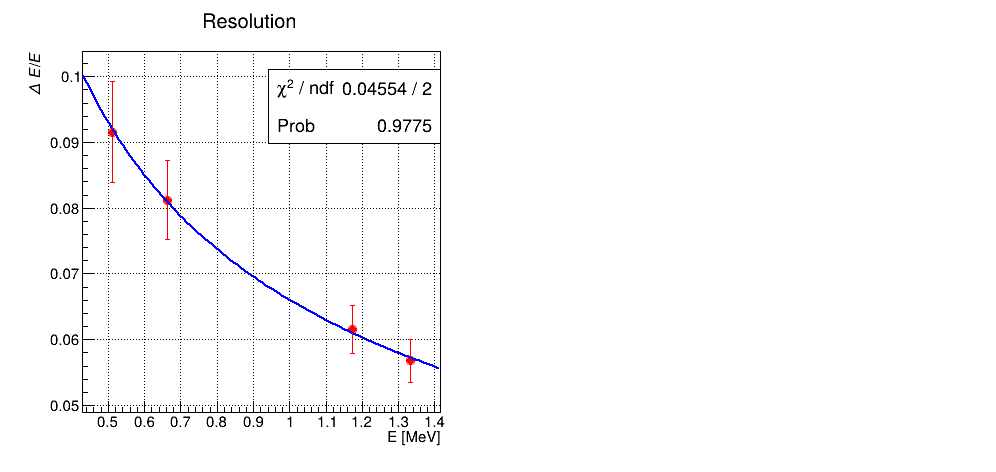
\includegraphics[scale=0.5]{images/energeticResolution.png}
\caption{Regressione con il modello (\ref{eq:resolution}) ai dati in \cref{tab:resolution} per caratterizzare l'andamento della risoluzione $ R = \Delta E / E $ del rivelatore contro l'energia $ E $.}
\label{fig:resolution}
\end{figure}

\begin{table}
    \centering
    \begin{tabular}{c|cc|cc|cc|cc}
        sorgente & $ E [\unit{MeV}] $ & $\delta E [\unit{MeV}] $ & centroide & $ \delta $ centroide & FWHM & $ \delta $ FWHM & $ R \qty(\frac{\Delta E}{E}) $ & $ \delta R $ \\
        \hline
        \ce{^22Na} & 0.5110 & 0.0010 & 307.2 & 1.5 & 27.1 & 0.7 &0.092 & 0.008 \\
        \ce{^60Co} - 1 & 1.1732 & 0.0010 & 685.0 & 1.5 & 41.2 & 0.7 & 0.062 & 0.004 \\
        \ce{^60Co} - 2 & 1.3325 & 0.0010 & 780.5 & 1.5 & 43.0 & 0.7 & 0.057 & 0.003 \\
        \ce{^137Cs} & 0.66166 & 0.00010 & 395.4 & 1.5 & 31.0 & 0.7 &0.081 & 0.006 \\
    \end{tabular}
    \caption{Dati relativi al fit in \cref{fig:resolution}: abbiamo usato i valori di energia teorici $ E $, e li abbiamo confrontati con la FWHM in energia per ogni picco calcolata a partire dalla FWHM in canali (stimata dal software). Abbiamo usato come errori sulle stime dei centroidi e della FWHM le deviazioni standard delle misure ripetute di \ce{^60Co}.}
    \label{tab:resolution}
\end{table}

\section{Misura dell'attività di una sorgente}

Abbiamo acquisito gli spettri di due sorgenti di \ce{^137Cs} (etichettate FS65 e FS66) per determinarne l'attività, sia con un metodo relativo che con uno assoluto.

\begin{figure}[]
    \centering

    \subcaptionbox{Sorgente FS65 \label{fig:fs65}}
    {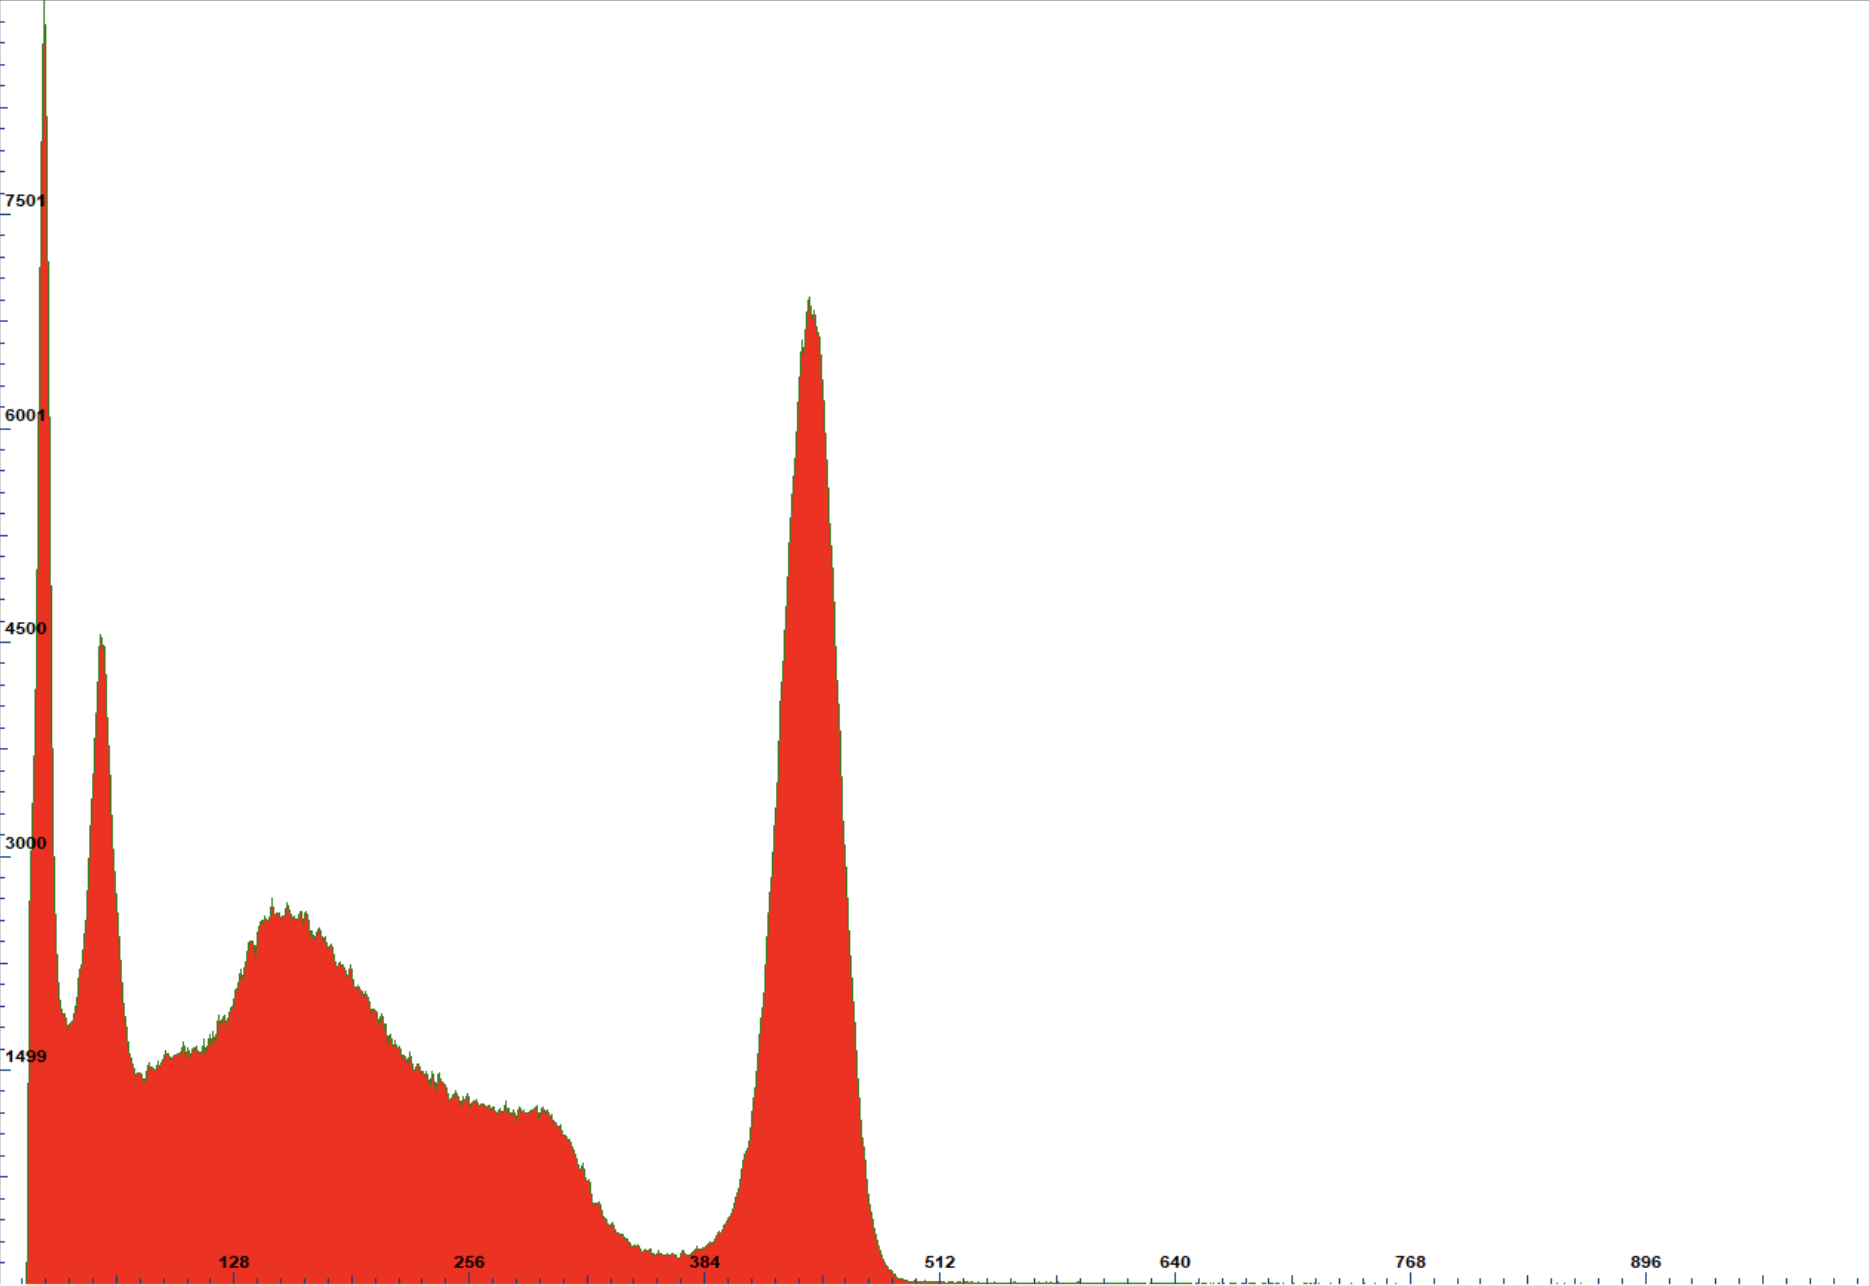
\includegraphics[width=0.45\textwidth]{images/fs65.png}}
    \hfill
    \subcaptionbox{Sorgente FS66 \label{fig:fs66}}
        {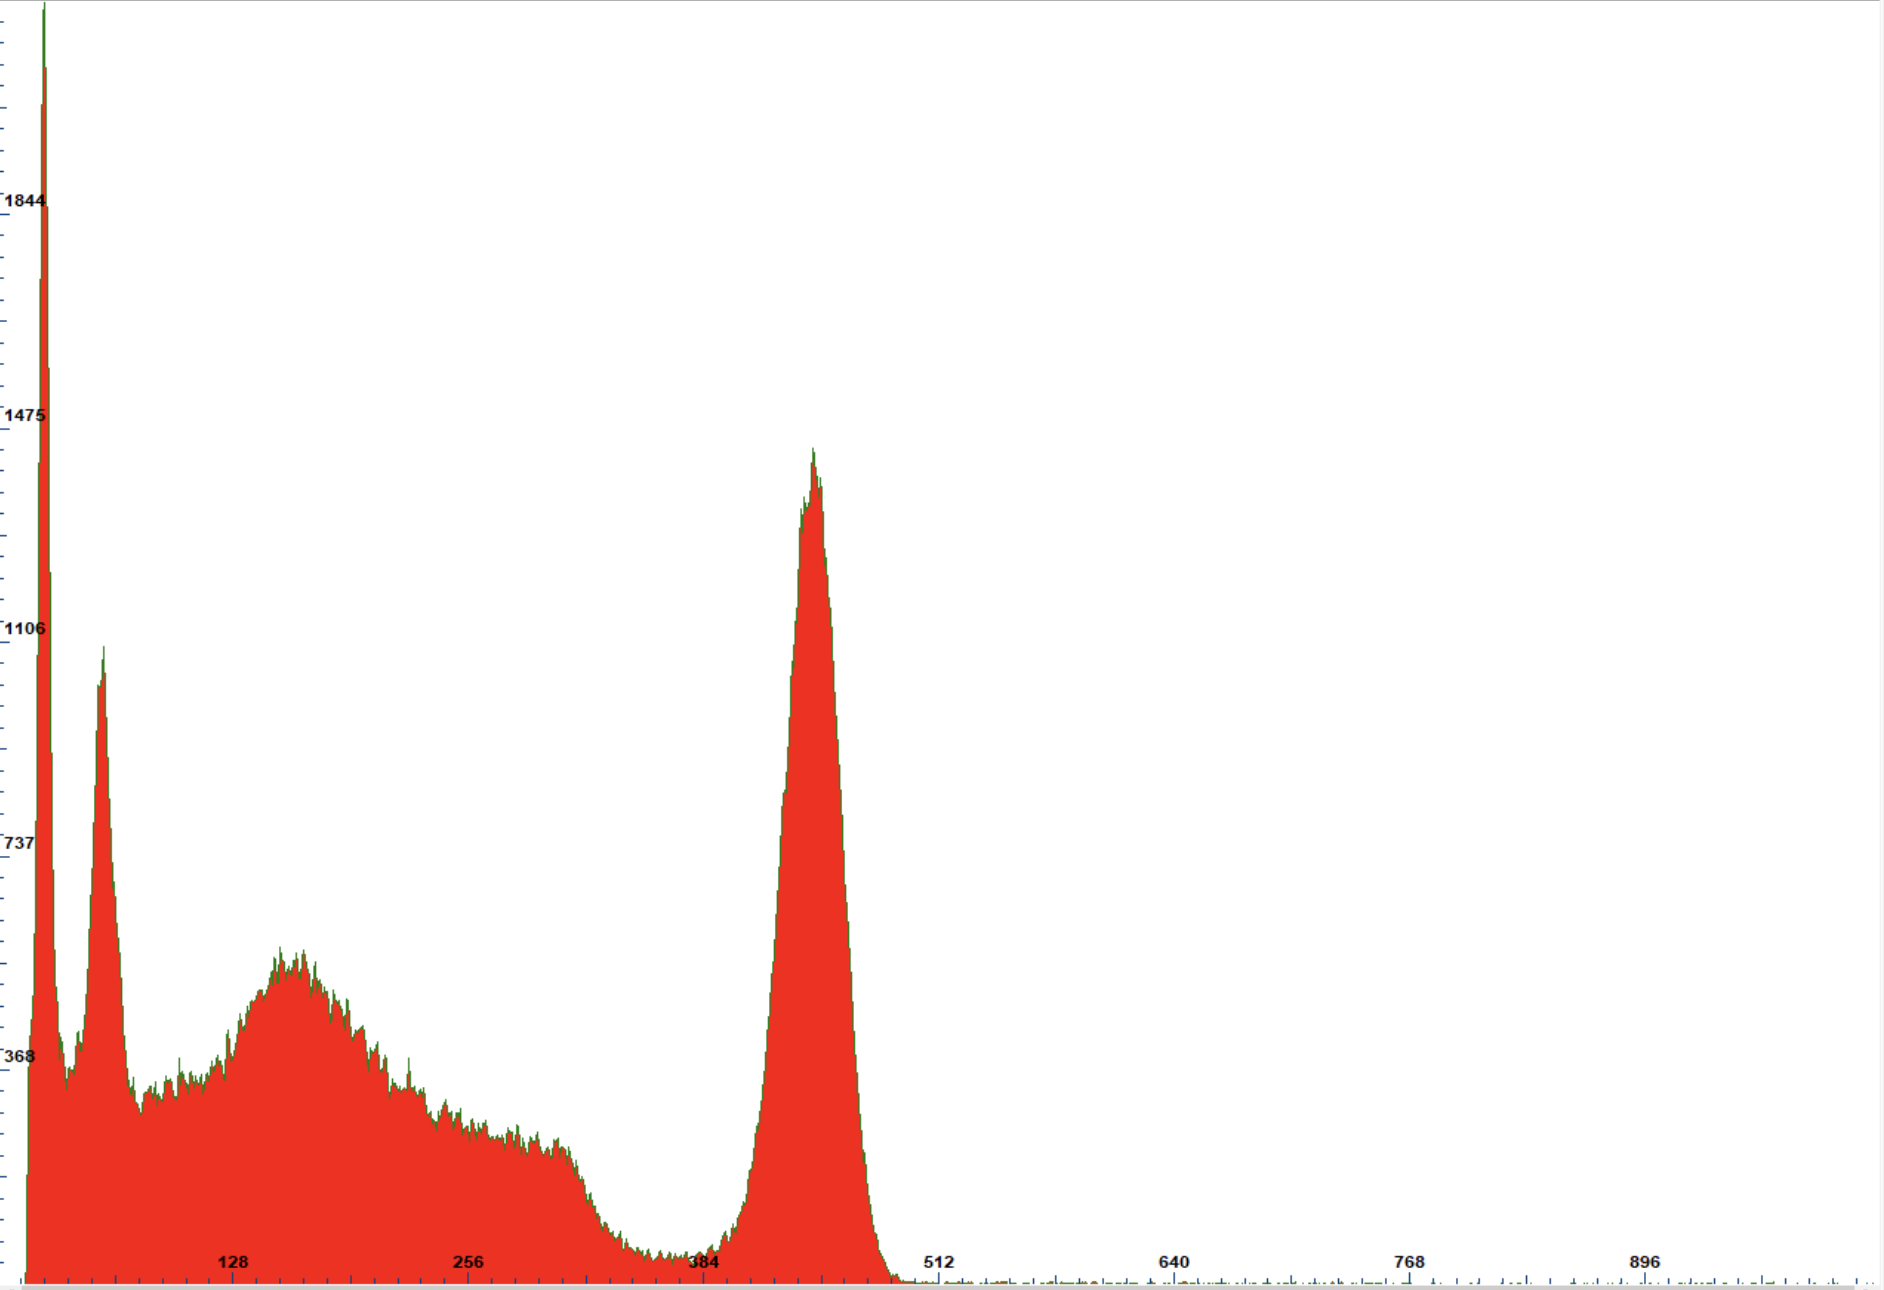
\includegraphics[width=0.45\textwidth]{images/fs66.png}}

        \caption{Spettri delle sorgenti di \ce{^137Cs} FS65 e FS66 di cui abbiamo determinato le attività. Anche se i tempi di misura $ t_\text{live} $ sono pressoché identici l'altezza del picco della sorgente FS65 è chiaramente maggiore di quella della sorgente FS66 (le scale degli assi verticali sono diverse nei due grafici).}
    \label{fig:activityspectra}
\end{figure}

Le attività nominali delle sorgenti sono note al 07/11/2024:
\begin{equation}
A_\text{FS65} = (193 \pm 10)\unit{kBq} \qquad  A_\text{FS66} = (37.4 \pm 1.9) \unit{kBq}
\end{equation}
e considerando il tempo di dimezzamento del \ce{^137Cs}:
\begin{equation}
t_{1/2} = (30.150 \pm 0.010) \unit{y}
\end{equation}
abbiamo utilizzato la legge di decadimento esponenziale per calcolare le attività tabulate al giorno dell'esperienza (14/04/2026, cioè $ \Delta t = (1.432 \pm 0.003) \unit{y} $):
\begin{equation} \label{eq:expdec}
A = A_0e^{-\lambda\Delta t}
\end{equation}
ottenendo:
\begin{equation}\label{eq:csactivities}	
A_\text{FS65,today} = (187 \pm 9) \unit{kBq} \qquad A_\text{FS66,today} = (36.2 \pm 1.8) \unit{kBq}.
\end{equation}

In particolare, per applicare entrambi i metodi abbiamo misurato i rate dei picchi fotoelettrici delle due sorgenti stimandoli usando:
\begin{equation}
R = \frac{A_n}{t_\text{live}}
\end{equation}
come riportato in \cref{tab:csrates}, dove $ A_n $ è il numero di conteggi netti (con errore calcolato a partire dai conteggi lordi $ A_g $ come illustrato in \cref{sec:errnetcounts}) e $ t_\text{live} $ il tempo di misura a cui è stato sottratto il tempo morto. 

\begin{table}
	\centering
	\begin{tabular}{c|cccccc}
		sorgente & $A_n$ & $A_g$ & $t_\text{live} \, [\unit{s}]$ & $\delta t_\text{live} \, [\unit{s}]$ & $R \, [\unit{s^{-1}}]$ & $\delta R \, [\unit{s^{-1}}]$ \\
		\hline
		FS65 & 257764 & 273300  & 349.150 & 0.010 & 738.3 & 1.5 \\ 
		FS66 & 51439 & 55415 & 354.170 & 0.010  & 145.2 & 0.7 
	\end{tabular}
	\caption{Dati relativi al conteggio dei rate del picco fotoelettrico delle due sorgenti di \ce{^137Cs}: l'area netta del picco $A_n$ determinata dal software rimuovendo il background all'area lorda $A_g$ (espresse entrambe in numero di conteggi), il tempo di misura $t_\text{live}$ e i rate con il loro errore.}
	\label{tab:csrates}
\end{table}

\subsection{Attività della sorgente con il metodo relativo}

Il metodo relativo ci permette di ricavare l'attività di una sorgente incognita (FS66) conoscendo quella di una sorgente nota (FS65) sfruttando la proporzionalità diretta tra attività e rate di conteggi $ A \propto R $:
\begin{equation}
A_x = A_s\frac{R_x}{R_s}.
\end{equation}	

Quindi, usando i dati in \cref{tab:csrates} abbiamo calcolato l'attività della sorgente FS66:
\begin{equation}
A_\text{FS66,rel} = (36.8 \pm 1.9) \unit{kBq} 
\end{equation}
e confrontandola con quella teorica in \cref{eq:csactivities} con un test Z abbiamo trovato che è compatibile ($ Z = 0.207 $ e $ p = 0.836 $) al 5\%.

\subsection{Attività delle sorgenti con il metodo assoluto}

Per utilizzare il metodo assoluto sfruttiamo la relazione seguente:
\begin{equation}\label{eq:absactivity}
	A = \frac{R}{\epsilon G f_g}
\end{equation}
dove $R$ sono i rate, $\epsilon$ è l'efficienza del rivelatore, $G$ è l'accettanza mentre $f_g$ è la frazione di decadimento.
In particolare abbiamo calcolato $G$ con la seguente relazione:
\begin{equation} \label{eq:acc}
G = \frac{1}{2}\qty[1-\cos(\arctan(\frac{a}{d}))].
\end{equation}

Nello specifico nel nostro setup:\footnote{Il valore dell'efficienza $\epsilon$ dipende sia dall'energia dei $\gamma$ incidenti, sia da fattori geometrici: questa stima è valida per il picco di emissione del \ce{^137Cs} alla distanza $ d = 9.3 \unit{cm} $.}
\begin{equation}
\epsilon = (0.25 \pm 0.01) \quad f_g = 0.851 \quad a = (2.5 \pm 0.1) \unit{cm} \quad d = (9.3 \pm 0.1) \unit{cm}
\end{equation}
e quindi abbiamo valutato l'accettanza come $ G = (0.0177 \pm 0.0013)$ (usando l'\cref{eq:acc}).

Usando l'equazione in \cref{eq:absactivity} con i rates in \cref{tab:csrates} abbiamo ricavato:
\begin{equation}
A_\text{FS65,abs} = (196 \pm 17) \unit{kBq} \qquad A_\text{FS66,abs} = (38\pm3) \unit{kBq}
\end{equation}
Valori che se confrontati con quelli in \cref{eq:csactivities} con un test Z risultano essere compatibili ($Z_{65} = 0.727$, $ p_{65} = 0.467$ e $Z_{66} = 0.956$, $ p_{66} = 0.399$) al 5\%.  


\section{Determinazione del coefficiente di assorbimento di massa $ \mu / \rho $ }

Un fascio di raggi $\gamma$ monocromatico, attraversando uno spessore di materiale assorbente,\footnote{L'assorbimento di un materiale cresce al crescere della sua densità $\rho$ e del suo numero atomico $Z$.} viene attenuato secondo la legge:
\begin{equation}\label{eq:decay_false}
I = I_0 e^{-\mu x}
\end{equation}
dove $ \mu $ è il coefficiente di assorbimento lineare, $ \rho $ la densità del materiale e $ x $ lo spessore attraversato dalla radiazione.

In particolare, abbiamo utilizzato come unità di misura dello spessore $ X = \rho x $, pesando per la densità del materiale, in modo da avere l'equazione di Lambert-Beer (\ref{eq:decay_false}) come:
\begin{equation} \label{eq:decay}
I = I_0 e^{- \frac{\mu}{\rho} X}
\end{equation}
nei termini del coefficiente di assorbimento normalizzato per la densità $ \mu / \rho $.

Abbiamo acquisito cinque spettri di emissione per la sorgente \ce{^137Cs} variando lo spessore di piombo attraversato dai $ \gamma $ emessi con delle lastre di spessore $(2.1 \pm 0.1) \unit{mm} $ ciascuna.\footnote{In particolare abbiamo assunto come indipendenti gli errori sugli spessori delle lastre, propagandoli di conseguenza.}

\begin{table}
	\centering 
	\begin{tabular}{c}
	ciao
	\end{tabular}
	\caption{}
	\label{tab:csassorbim}
\end{table}

Sui dati in \cref{tab:csassorbim} abbiamo effettuato una regressione con il modello in \cref{eq:decay} (in \cref{fig:absorb}) ottenendo come stime dei parametri: \help{insert data in table + fig}
\begin{equation}
	I_0 = (422 \pm 2) \unit{s^{-1}} \qquad \mu / \rho = (0.1040 \pm 0.0010) \unit{cm^2/g}
\end{equation}
e in particolare abbiamo confrontato $ \mu / \rho $ con il valore teorico:
\begin{equation}
	(\mu / \rho)_\text{true} = 0.1035 \unit{cm^2/g}
\end{equation}
effettuando un test Z che conferma la compatibilità tra i due dati (con $Z = 0.523 $ e $ p = 0.601 $) al 5\%. 

\begin{figure}
	\centering
	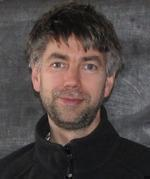
\includegraphics[scale=0.5]{./images/pacini}
	\caption{}
	\label{fig:absorb}
\end{figure}

\section{Analisi del picco somma nello spettro del \ce{^60Co}}	

Il \ce{^60Co} emette raggi $ \gamma $ a due energie distinte: abbiamo provato a determinare se queste due emissioni avvengono in maniera indipendente (sono prodotte da decadimenti indipendenti), oppure se fanno parte di un unico decadimento in cascata. 

In entrambi i casi, talvolta il rivelatore misurerà due eventi contemporaneamente (cioè in un tempo minore della sua risoluzione temporale $ \Delta t = (1 \pm 1) \unit{\micro s} $): nel multicanale verrà conteggiato un evento con energia pari alla somma delle energie dei due $ \gamma $, che contribuirà a formare il cosiddetto picco somma.

La frequenza di queste osservazioni ``doppie'', però, dipende dalla correlazione/scorrelazione tra i due eventi.
Assumendo che i conteggi (netti) nel picco somma $ \Sigma_\text{dep} $ e $ \Sigma_\text{ind} $ siano piccoli rispetto a quelli (sempre netti) nei fotopiccchi $ \Sigma_1 $ e $ \Sigma_2 $, abbiamo che:
\begin{equation}
\Sigma_\text{dep} =\frac{\Sigma_1 \Sigma_2}{At_\text{live}} \qquad \Sigma_\text{ind} = \frac{\Sigma_1 \Sigma_2 \Delta t}{t_\text{live}} 
\end{equation}
dove $ A $ è l'attività della sorgente, $ t_\text{live} $ il tempo di acquisizione (a cui è stato sottratto il tempo morto), e $ \Delta t $ la risoluzione temporale del rivelatore. 

In particolare, abbiamo ricalcolato l'attività della sorgente (FS64) dal 7/11/2024 al 15/04/2026 (con la legge di decadimento esponenziale \cref{eq:expdec} con $ \Delta t = \ldots $): \help{insert precise time w/ error + activity is obv wrong}
\begin{equation}
A_\text{FS64} = (39.2 \pm 2.0) \unit{kBq} \qquad A_\text{FS64,today} = (32.460 \pm 0.084) \unit{kBq}.
\end{equation}

\begin{table}
	\centering
	\begin{tabular}{c}
		ciao
	\end{tabular}
	\caption{}
	\label{tab:cspeaksum}
\end{table}

In particolare, abbiamo misurato lo spettro due volte (variando leggermente il setup sperimentale, ma con la stessa sorgente) e in entrambi i casi abbiamo trovato (i dati sono raccolti in \cref{tab:cspeaksum}) che i conteggi effettivamente misurati nel picco somma $ \Sigma_\text{sum} $ non sono compatibili né con $ \Sigma_\text{dep} $ né con $ \Sigma_\text{ind} $.
Ad ogni modo, l'ipotesi di un decadimento a cascata produce una stima che ha lo stesso ordine di grandezza dei conteggi misurati, mentre quella di decadimenti indipendenti no.
Questo suggerisce fortemente che l'ipotesi di decadimenti correlati sia più probabile, ma che per ottenere delle previsioni più precise si debbano considerare delle approssimazioni meno grossolane.


\section{Conclusioni}

Con questa esperienza abbiamo potuto studiare lo spettro di emissione gamma di alcuni isotopi radioattivi e la loro attività.  
\help{INSERIRE PARTI CONCLUSIVE}
L'analisi delle sorgenti $FS65$ ed $FS66$ di \ce{^60Cs} ha portato a risultati compatibili con quelli attesi sia utilizzando il metodo relativo che quello assoluto. 
\begin{equation}
	A_{FS66\text{rel}} = (36.8 \pm 1.9) \unit{kBq}
\end{equation}	
\begin{equation}
	A_{FS65\text{abs}} = (196 \pm 17) \unit{kBq} \quad A_{FS66\text{abs}} = (38 \pm 3) \unit {kBq}
\end{equation}
Successivamente si è ricavato il coefficiente di assorbimento di massa del piombo che è risultato essere statisticamente compatibile con il valore teorico.
\begin{equation}
	\mu /\rho = (0.1040 \pm 0.0010) \unit{cm^2/g} 
\end{equation}
Infine, ci siamo preoccupati di studiare il picco somma del \ce{^60Cs} in modo da poter determinare se gli eventi nel picco fossero correlati o se avvenissero in maniera indipendente. L'attività trovata in laboratorio risulta essere incompatibile con entrambe le ipotesi. 
\begin{equation}
	A_{FS64\text{today}} = (32.5 \pm 1.7) \unit{kBq} 
\end{equation}
\help{Come risultato di questa misura io ho messo l'attività ma non penso sia corretto, ha più senso mettere i valori di $\Sigma_1$ e $\Sigma_2$?}
Tuttavia il risultato suggerisce che il decadimento sia a cascata visto che i due valori hanno lo stesso ordine di grandezza. 


\clearpage

\appendix

\clearpage

\bibliographystyle{plain}

\bibliography{references}

\end{document}
